  
\documentclass[11pt]{article}  

\usepackage{ifpdf}
\ifpdf 
    \usepackage[pdftex]{graphicx}   % to include graphics
    \pdfcompresslevel=9 
    \usepackage[pdftex,     % sets up hyperref to use pdftex driver
            plainpages=false,   % allows page i and 1 to exist in the same document
            breaklinks=true,    % link texts can be broken at the end of line
            colorlinks=true,
            pdftitle=Proposal
            pdfauthor=Hamoun Ghanbari
           ]{hyperref} 
    \usepackage{thumbpdf}
\else 
    \usepackage{graphicx}       % to include graphics
    \usepackage{hyperref}       % to simplify the use of \href
\fi 
\usepackage{setspace}
\doublespacing

\title{Model-Based Dynamic Resource Management For Multi Service Information Systems}
\author{Hamoun Ghanbari}
\date{}

\begin{document}
\maketitle

	\begin{abstract}
	\footnotesize
	Cloud computing provides the computational power of data centers to a large user community over the web. In Software as a Service (SaaS) and Platform as a Service (PaaS) forms of the cloud, multiple high-level services and end-user applications are hosted on the cloud provider's available resources.
A major problem for SaaS and PaaS cloud providers, is associating the optimal amount of physical hardware to services. The optimality of this association is measured in terms of meeting the promised Quality of Service (QoS) for the applications while minimizing the overall infrastructure cost. 
We target solving two variations of this problem using model-based control. We model the cloud infrastructure, the services, and the applications using the Layered Queuing Models (LQM). 
To build and maintain such models we use an existing estimation technique called Kalman Filtering (KF).
%
In our first contribution, we improve the convergence of the existing Kalman Filter based estimation for large LQM models. This is done by dynamically clustering the applications into a smaller set. This improves the convergence of the estimation while keeping the modeling error at an acceptable level.
%
The second problem involves the allocation of limited resources to a set of applications by tuning the fraction of resource capacity allocated to each application.  

The optimization used in this case, works best when there is no restriction, guideline, or associated cost on the number of reconfigurations. 
%
In presence of such restrictions, this approach can create overhead and perturbations for the running applications.
To alleviate the above problem, in our third contribution, we propose a dynamic service placement algorithm that considers the trashing cost in calculating the optimal configuration using Model Predictive Control (MPC). Through experiments, we validated our hypothesis that model predictive approach performs better than the simple stepwise optimization when the objective functions are long term and when trashing is taken into account. 

% The goal is to dynamically tune a data driven regression model. 
	\end{abstract}
	
 \section{Introduction}   
 Cloud computing provides the computational power of data centers (e.g., network, storage, computational devices, and services) to a large user community over the web. 
	 A cloud is formed by an interconnected set of datacenters. 
	 A data center environment is composed of a communication system, servers, and astorage subsystem. 
	 These computing resources are hosted in controlled environments and under centralized management. 
		Currently there are three types of cloud computing offerings: Infrastructure as a Service (IaaS), Platform as a Service (PaaS), and Software as a Service (SaaS). 
		IaaS multiplexes the hardware layer and offers computing services such as storage, CPU and memory to users. 
		In SaaS and PaaS, multiple higher-level services and end-user applications are hosted on Cloud provider's available resources. 
		A PaaS provider is an enterprise that is responsible for leasing application environments or programmable services to customers for various durations of time. 
		Customers of PaaS could deploy their own programs on purchased platforms from a PaaS provider. 
		SaaS type of Cloud provides instances of software and applications that are typically installed in businesses' computer networks or personal computers. 
		Examples of this software include customer relationship management (CRM), accounting, invoicing, human resource management (HRM), and content management (CM). 
		Because SaaS and PaaS host services, they are sometimes referred to as Multi Service Information System (MSIS)\cite{li2011fast}, application service centers, or service centers in short.  
		
  A major problem for SaaS and PaaS cloud providers is associating the optimal amount of physical hardware (including CPUs, networks, etc.) to services. 
  The amount of the physical hardware is fulfilled by choosing the optimal deployment and resource share of the services on the available hardware.
	%, and the optimal resource share for each service replica.  
	This problem is generally known as Optimal Service Placement (OSP)\cite{zhang2012dynamicPlacement}. 
   For OSP, the optimality is measured in terms of meeting the promised Quality of Service (QoS) mentioned in Service Level Agreement (SLA)\footnote{Formally, a SLA is a contract which defines the relationship between a service provider and its clients that fully specifies all obligations for both parties, the price to be paid for the service(s) offered and associated penalties should obligations be unmet. It can be quite complex and comprehensive (e.g., considering aspects of both functional and non-functional requirements); however, in this work, only performance objectives that can be extracted from an SLA are considered. No attempt is made to fully model or develop an SLA or an SLA management framework.} while minimizing the overall cost. SLAs include a set of performance metrics experienced by applications or classes of customers\footnote{A class of users in the context of this research is composed of a set of users that access the system services using the same pattern.}.
	Performance metrics usually represent time behavior of the services such as average throughput, mean response time, total percentage of requests rejected or not handled within certain time limit. 
	In a PaaS and SaaS, the cost is associated with the number of active hardware components contributing to the cost of electricity and cooling. 

In the remainder of this section, we present the fundamentals and assumptions of our work. Subsection \ref{sec:model_based_resource_management_architecture} presents the model-based approach to resource management. Subsection \ref{sec:layered_queuing_model} presents our model for the service center.
 
\subsection{Model Based Resource Management Architecture}  
\label{sec:model_based_resource_management_architecture}
 %The approach we propose to address the OSP problem is using a model-based feedback loop.
  A solution to an OSP problem is a sequence of feasible allocation actions over time that maximizes a defined performance criterion (or an objective function) regarding SLAs\footnote{One can instead say the optimal control minimizes an expected total cost function}.
In our approach, these allocation decisions are made at each time-step based on the information available from the system up to that time.
 A controller constantly considers the most recent monitored data for calculating the proper actions. Thus, the original plan is adjusted according to the new observation samples of the environment in the past step. This is called the feedback based scheme or closed loop control.

 The model-based feedback loop we propose is based on the IBM's MAPE-K loop architecture, which is composed of the following four subsystems: a monitor, an analyzer, a planner and an execution subsystem.
Figure \ref{fig:mapk_loop} represents the schematic view of the IBM's MAPE-K loop.
	\begin{figure}
		\centering
			\includegraphics{images/mapk_loop.pdf}
		\caption{Schematic view of the IBM's MAPE-K loop.}
		\label{fig:mapk_loop}
	\end{figure}
	
 The Monitoring subsystem is responsible for measuring inputs, and outputs of the managed system, quantifying them, sometimes aggregating them, and keeping them as a history.
In our case, the monitored metrics are the service specific performance metrics for different types of server processes (e.g. load balancer, web server, application server, and database server).

   The analyzer subsystem, identifies and tunes a model of the system under management, and estimates the unobservable portion of system state. The model enables the planner to project the system's behavior and the state under different actions in the future.   
   Queuing theory based models \cite{petriu_approximate_1994,petriu_approximate_2004,badidi-queuing-2005} and Layered Queuing Models (LQM) \cite{rolia_method_1995,ramesh_multi-layer_1998} developed upon Mean Value Analysis (MVA) of queuing networks have been widely used to capture the behavior of multi-tier distributed applications \cite{litoiu_hierarchical_2005, xu_performance_2006,hamoun_ghanbari_tuning,liu_layered_????}. 
They can be utilized to describe the expected performance of service centers (i.e. response time and throughput) in relation to various inputs.  A major concern is the ability to synchronize the model based on the observed behavior of the system. In our case, the analyzer uses statistical techniques to maintain an up-to-date LQM.
 
   A planner uses the model to rapidly explore multiple decisions and find near-optimal solution towards a goal \cite{litoiu_hierarchical_2005,aiber2004autonomic}. 

   A execution subsystem applies the derived control actions to the system.
  
   \subsection{The LQM Based Cloud Model} 
	\label{sec:layered_queuing_model}
	 A service center can be modeled by a set of queues where devices are mapped to queuing or delay centers.  Based on the physical structure of the data center and the service invocations, one can build a queuing networks model. Then, a general Mean Value Analysis (MVA) of the model can be used to calculate the performance characteristics of the system. 
\begin{figure}[htbp]
\begin{center}
	\includegraphics[scale=0.5]{images/cloud_queuing_model}
	\caption{A simplified view of LQM, which is used to model a service center. The dashed line denotes the separation between software and hardware layers.}
	\label{fig:cloudQueuingModel}
	\end{center}
\end{figure}


	 % The workload of applications are the service requests made by end-users through protocols such as HTTP. 
	  Workload of a service is driven by its external users hence usually quantified by number of users and think time or request arrival rate, which is measured in requests per seconds. Each group of users uses the services and the resources in a different way (for example with highly different CPU demands). Thus it is common to refer to each group as a different \textit{class}. In multi-class queuing models, outputs are given in terms of the individual customer classes. It is therefore reasonable to model each application with a separate class of users with a fixed population. 
	 CPU is the main resource accessed by services. Other resources such as hard disks and network are used from CPU. 

	% In queuing models, the way services interact with hardware resources is quantified in terms of service times.  The service time is the time each request spends on each resource type when the service is invoked.
A simplified view of LQM which is used to model a service center is presented in figure \ref{fig:cloudQueuingModel}. Figure \ref{fig:service_call_graph} demonstrates an example of a service center, composed of 14 services (denoted by s1 to s14), accessed by 2 classes of users (the two rectangles at the top). The figure represents the call graph of the services, the think times ($Z_c$), the number of users ($N_c$) of each class over time, and the invocation numbers within services (i.e. the numbers placed beside the arrows). 
As an example, here we give one interpretation for the model.
Assume s3 is an accounting application, and s6 is a database service.
Every request of the accounting application on average invokes the database service 2.5 times.
There are two organizations using the accounting application. Initially organization1 has 250 users and organization2 has 100 users. On each round of visit to the service center\footnote{The model is flexible in terms of defining the `round of visit'.} organization1 invokes application once and organization2 invokes the application twice. 
	\begin{figure}[htbp]
\begin{center}
 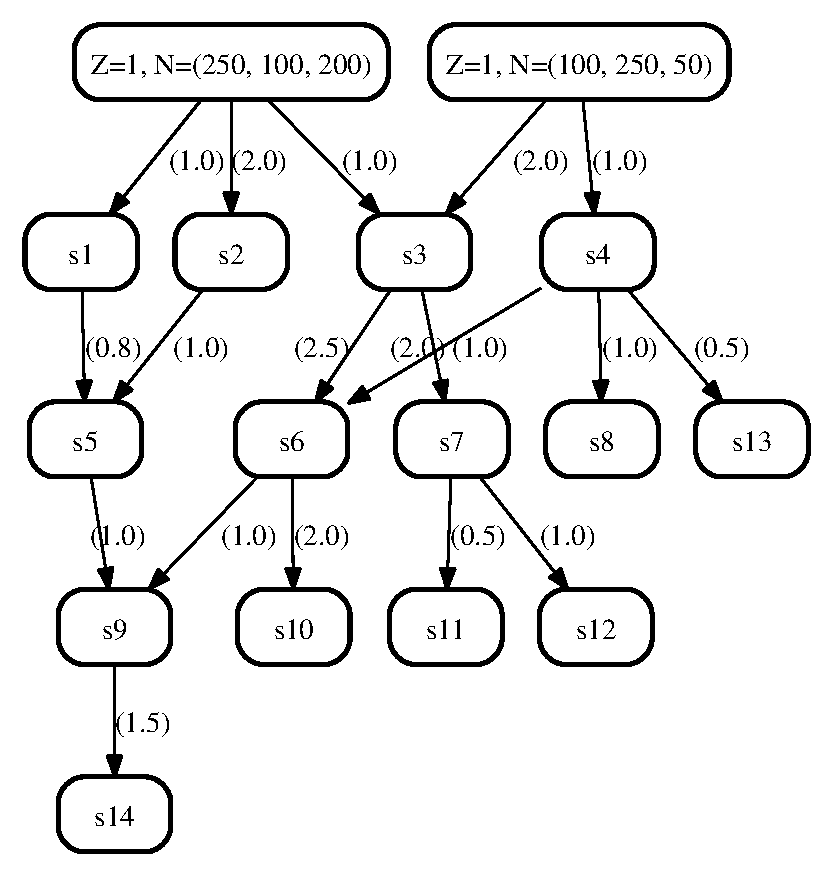
\includegraphics[scale=0.8]{images/example1services}
\caption[An example small scale service center]{An example small scale service center: the call graph of services and classes, the think times $Z$ and number of users $N$ of each class over time (e.g. 250, 100, 200 is the number of users for the next three steps for the class 1). The edges between services represent invocations between services, and the numbers placed beside these ages represent the number of invocations. The edges between classes and services represent visit ratios. }
\label{fig:service_call_graph}
\end{center}
\end{figure}
% There are 6 available hosts to support the services. Capacity of the hosts are  $\capp=[16\ 6\ 6\ 16\ 6\ 6]^T$

	 \subsubsection{Application scaling and optimization through service replication} 
	An important tool in controlling the performance of applications is to adjust the amount of resource given to their services.
	Through replication, each service can be distributed across multiple physical machines. Each instance of a service is then called a replica. Each replica will handle a portion of the original service's workload.  The actual demand on each resource is obtained by taking into account this association.
	
 One can adjust the load on each replica by distributing the accesses to replicas in a desired proportion.
In fact, in our third contribution, we use optimization to determine the number of replicas, allocation of the replicas to physical machines, and the amount of load on each replica. 

 \section{Contribution 1: Improving The Convergence Of Performance Model Estimators using Dynamic Clustering of User Classes} 
% Tracking Adaptive Performance Models
\label{models_in_a_state_estimation} 
%The first contribution of this thesis is a method for improving the convergence of Bayesian approach to performance model estimation.
 The LQM model described earlier, needs to be built based on the measurement data. This requires that the service demands and the workload parameters be estimated for each class of users.
 Bayes filters have been successfully applied to perform this task~\cite{woodside_use_2005,xu_performance_2005,zheng_tracking_2005}.
Despite effectiveness, an important issue in using the Bayesian approach is convergence.
 Bayes filters do not converge to a solution unless we have more measured parameters than estimated state parameters. Therefore, the number of classes should be reduced to a certain size, hugely reducing the scalability of the estimation to model large data centers.

We propose the clustering of user classes into a smaller set with lower cardinality, therefore increasing the scalability of Bayesian performance model estimation. 
By decreasing the number of classes, we also reduce the amount of computation the estimator has to perform.
However, by grouping the classes we introduce some modeling error\footnote{Modeling error is the mismatch of model output and the monitored metrics.
It comes from the fact that the service demands are now represented using fewer parametrized statistical distributions. Note that this modeling error is a measure that we introduced. The Bayesian filter already tries to minimize the weighted cumulative sum of process noise and the observation noise over infinite horizon of time. However, the modeling error that we define here is more a heuristic measure to compare two different groupings of classes over a very limited time horizon. }.
That is the reason we cannot cluster all the classes as into one group. We propose an algorithm to determine the best choice of the number of clusters and the grouping of classes into these clusters, in a way that the estimation converges at the same time we have a low modeling error. The major contribution of our approach is, thus, dynamic clustering of user classes, to improve the convergence of the filter and yet leave enough classes to satisfy the accuracy criterion.  

In the paper \cite{hamoun_ghanbari_tuning}, we validated the method with a set of experiments on a deployed web application. The first set of experiments were tracking the service demand of a web application.  
We tested if the algorithm could maintain the same upper bound on the modeling error by dynamically changing the number of clusters over the experiment. The test was passed successfully; for a given modeling error percentage the algorithm could maintain the same modeling error by adjusting the number of clusters. For example, it could reach 17\% error using only 60\% of the original classes. % The actual number of classes oscillated between 7 and 12 for the duration of the experiment.
 
We also performed the same test for a case where the service demands change at different rates and phases in short run. The system under test was a simulated web based e-commerce site. We observed that our estimation and classification algorithm works quite well, since it is able to keep the error below 8\% with the smallest number of clusters and acceptable frequency of re-clustering. 

  To the best of our knowledge, the combination of dynamic clustering and parameter estimation has never been investigated before. The only related work in terms of final goal is \cite{sharma_automatic_2008}. They try to categorize requests based on their resource usage characteristics. However, they ignore the prior knowledge about requests in the system and classify the requests on the fly. Thus, their utilized approach is also different, as they use a machine learning technique called Independent Component Analysis (ICA). 

 \section{Contribution 2: Optimal Resource Share Adjustment in Cloud Using Dynamically Tuned Empirical Models}    
% Resource Share Adjustment in Cloud with no Reconfiguration Cost
% Performance Model Estimation and Tracking using Optimal Filters
\label{optimization_no_reconfiguration_cost} 
 A major research problem in the area of application service centers involves the allocation of limited resources to a set of applications where applications are deployed on virtual machines (VMs). In a virtualized data center, this can be done by tuning the fraction of resource capacity allocated to each application's VM. 
Deriving the optimal set of resource fractions is usually done by optimizing a monolithic objective function based on the desired performance of applications. Necessary for this optimization, is a model of the application service center. The model can be either first principle (e.g. based on queuing theory) or be driven empirically from a data set.
% In the empirical approach, the model is obtained by an off-line regression analysis of applications' performances. 
 
A portion of the related work on optimal deployment such as \cite{li_fast_2009,li_performance_2009} assumes that the system follows an accurate first principle model. They suggest using a filter-based approach such as \cite{zheng-integrated-2011} to adaptively estimate the parameters of this model.
However, there is no guarantee that these first principle models accurately represent a service center, since it is usually very hard to model all aspects of a service center such as software contention, concurrency, remote calls, limited amount of memory, and limited amount of network bandwidth.  

On the other end, there is a major problem with the empirical models. 
% In terms of related work, the empirical model based approaches use regression analysis to discover their parameters. 
They do not propose a way to tune the models based on the measurement obtained during runtime.
When applications are deployed in the production environment, the original models start to show inaccuracy.
This is mainly because the deployment conditions are different from the test environments, which are used to build the training data sets.  
 
Our contribution is to increase the accuracy of the empirical models by tuning them dynamically using the measurement data at runtime on the fly. We also trace this in the overall performance of the allocation. We investigate if a model, built off-line through a nonlinear regression and dynamically tuned through an Extended Kalman Filter, can outperform the one that is not tuned. The other differences between our approach and the related work are the use of the decomposed models, and a custom optimization routine to optimize the defined utility functions.   

% "`The primary requirement of filtering algorithms such as Particle Filter (PF), Unscented Kalman Filter (UKF) and Extended Kalman Filter (EKF) is the availability of an accurate nonlinear state space model."'
In \cite{ghanbari_feedback-based_????}, we successfully tested the contribution. We simulated
a small cloud configuration with multiple instances of applications deployed on physical machines using CloudSim~\cite{CLOUDSIM2010}.
% A data set of the sample application's performance was generated synthetically by invoking the CloudSim simulator. A non-linear model derived from the mean value analysis for open queuing networks \cite{lazowska_quantitative_1984} was extended to account for capacity. A regression analysis was then performed on the resultant data, allowing model parameters to be computed.
We showed static non-tuned models of the applications results in a suboptimal allocation decision for some applications and leads to failure in meeting their SLAs. In contrast, using dynamically tuned models results in a more efficient resource allocations being made and better commitment to SLAs and better utility. 
We have to mention that, in the experiments, to lower the complexity of the experiments, we assumed that the capacity of the hosts, the workload intensities, and the service demands are either monitored or directly obtained; thus, the only quantities to be estimated (i.e. tuned) are the regression model coefficients.


% Our approach achieves the adaptation by tuning the model parameters using EKF.
% We are aware of the Expectation Maximization (EM) approach that separates the hidden states and the unknown parameters of a parametric state-space model and estimates them in a joint framework. However, we have not seen any instance of resource allocation context that uses such approach. 






% \cite{zheng-integrated-2011} for example this guy tries to estimate the parameters of (i.e. coefficients of) an state space model as well as estimating the hidden states at the same time. In this work, the parameters reside in the state transition equation rather than output equation. In the state space model, the state transition equation is linear but the parameters are unknown. The output equation, which is based on the first principle a queuing model, is nonlinear but the parameters are known. 

%\cite{soror_automatic_2010} targets a Pareto-optimal solution, a good trade-off between conflicting performance and cost-saving goals. Also the idea of dynamically adjusting the resource shares of multiple applications in order to meet a specified level of service differentiation, was used in \cite{liu_optimal_2007} and \cite{lim_automated_2009}, although using adaptive multivariate controller and for a more limited scenario than ours (i.e. maximum one PM per application layer).

% To derive the optimal fractions, one can model the whole service center as a LQM (taking each application as a class) and optimize over this model. Building such model requires estimating a large number of parameters proportional to the number of applications times number of services times number physical machines. Because of this, large monolithic models\footnote{A model that covers the whole data center, including all physical machines and services together.} cannot be really adapted in the scales of real service centers.
% Our first contribution is to decompose the monolithic LQM by assuming an individual model for each application. This assumption transforms the problem of estimating a single large LQM into estimating a large number of single class LQMs, thus highly reducing the complexity of the estimation. We do this by assuming applications are isolated in terms of the services they use. In other words, the set of services deployed for an application stays exclusive to that application. Through experiments, we show that such approach can be utilized to allocate resources in a midsize service center to a number of locations.


\section{Contribution 3: Optimal Service Replica Placement via Model Predictive Control} 
Application optimization through service replication and allocation can yield frequent changes in deployments (i.e. reconfigurations). 
The unnecessary frequent changes in the number of active servers or in the deployment of services on these service is usually referred to as trashing. 
Trashing can create overheads and perturbations for the running applications. 
Thus, if one of the objectives is to minimize trashing, reconfiguration, or service replica movement a typical static optimization (i.e. an optimization that does not consider time and only target one interval) does not work well. 
% It does not provide any way to distribute the changes over the next intervals to avoid trashing, overhead, and failure.

    To alleviate the above problem, we propose a dynamic service placement algorithm that considers the trashing cost in calculating the optimal configuration using Model Predictive Control (MPC). It solves a finite-horizon deterministic control problem at each control step. The solution of the optimization problem includes the number of service replicas, and optimal deployment of replicas on available hardware at each step. 

   Through experiments, we validated our hypothesis that the model predictive approach performs better than the simple stepwise optimization (e.g. an optimization that does not consider the future time such as the optimization performed in the second contribution) when the objective functions are long term and when trashing is taken into account. The result is represented in the paper \cite{ghanbari2014mpc} which is in the review process. 
  
		The most notable related work to this contribution is \cite{zhang2012dynamicPlacement}. It targets optimal service placement in geographically distributed clouds with reconfiguration cost taken into account through MPC. However, it has two main differences from our proposal: (i) it uses a single class open queuing network model, which is much simpler than the closed multi-class model we propose. (ii) It derives an analytical solution to a steady state version of the problem first and then targets this solution as a desired state through MPC with a quadratic trashing stage cost. In our case, this was not possible because we needed a sparse deployment at each step. A sparse deployment is one that most of services do not have replicas on most of the physical machines (i.e. the deployment matrix has many zeroes). For this reason, we had to use the sum of absolute values of the individual cost elements (as opposed to some of their squares). 
		
	%	Other examples of using MPC that we are aware of, are:~\cite{baiefficient,abdelwahed2004control, kandasamy2004self, bhat2006enabling,patikirikorala2011hammerstein}. However, they do not tackle the same problem as ours. In \cite{baiefficient,abdelwahed2004control,kandasamy2004self} MPC is used for managing a web server power consumption by changing the frequency at which the CPU is operating. Since, the number of choices of frequencies is quite small (i.e. less than 10 alternatives), changes in the frequency are trivial, and the feedback does not have a lot of delay. They were able to use a very small lookahead horizon and a simple model, and calculate the actual expected value of cost over noise ($w_j$) distribution, for every action path, without getting involved in a state explosion. In \cite{bhat2006enabling} MPC is used to decide about the amount of data each node of a cluster should send through a set of data streams, and the amount to cache to disks. The proposed solution maximizes throughput up to network congestion. In this paper, the choice of amount of data was continuous and the cost function was quadratic, which greatly helps with solving the MPC problem without any tricks or heuristics. 

 
  \section{ Thesis Outline}
     The following structure is proposed as the structure of this thesis. Each item in the list corresponds to a chapter in the thesis:  
    \begin{enumerate}
    
      \item \textbf{Introduction}. In chapter 1, we introduce the motivation and our approach. We motivate the three investigated problems in the thesis:
			Performance model estimation using dynamic clustering of user classes, optimal one-step-ahead resource share allocation for services, and optimal service replica placement via model predictive control.
			
    \item \textbf{Background}. Chapter 2 introduces the necessary background, including elements of autonomic control and adaptive systems, MAPE-K loop, optimal control theory, cloud computing, LQM, Bayesian estimation, and Kalman filter. 

  \item \textbf{Related Work}. Chapter 3 describes the state of the art that is relevant to the introduced problems. Regarding the first problem (i.e. service demand estimation), the related work is classified into three categories: linear regression, nonlinear regression, and Bayesian estimation. We then provide a literature review of the second problem (i.e. service resource allocation with no configuration cost). Third, we provide a literature review for the service replica placement problem considering the trashing cost. Since this is a new research topic, the related work is quite limited.
	 
  \item  \textbf{Models and State Estimation}.  
  Chapter 4 presents the first contribution, improving the convergence of the estimator by dynamic grouping of the classes of service. We introduce the concept of modeling error and propose a dynamic clustering algorithm to improve the convergence. Then we prove the applicability of the approach through a set of real experiments. We use the FIFA98 workload and the TPC-W benchmark for the experiments. We also perform a set of simulations to assess the result of the estimation and clustering algorithm for highly variable demands.  

\item \textbf{Optimal Resource Share Adjustment in Cloud Using Dynamically Tuned Empirical Models}. Chapter 5 discusses our solution for the case that there is no trashing costs. It investigates the use of decomposed LQM and a single step ahead optimization. 
We first formulate the problem, introduce the modeling and estimation, and then introduce the optimization process. The proposed approach will be assessed by two cases studies of different scales. 

   \item  \textbf{Optimal Service Replica Placement via Model Predictive Control}. 
 In chapter 6, we target the OSP problem where reconfiguration cost is taken into account. Then we discuss the solution to the problem via Model Predictive Control framework.  
In this chapter, we first introduced the notation and defined the problem.
We elaborate on the cost elements. 
There are a set of challenges in solving the introduced problems, including the non-linearity of the LQM, and the non-linearity of the infrastructure cost.
We then discussed the fast (but not the exact) solution to the problem. The solution is transformed into a solver friendly format that can be handled by a common convex optimization solver such as \texttt{cvx}.

We then explain the solution that considers the effect of the contention
We show the behavior of the resulting optimization in a set of experiments using the FIFA98 workload and a synthetic service center. In a second set of simulations, we investigate the effect of lookahead horizon in the performance of the control. This will be done through several cost trade-off curves that compares the variation of the cost factors (i.e. the cost of SLA violations, the cost of resource, and the cost of trashing) four different look ahead horizons.
 %   \item  \textbf{Optimal Service Placement in a Virtualized Environment}
 %  In chapter 6, we first formally introduce the optimal autoscaling problem in virtualized environment and describe how it is related to OSP. We introduce a currently known sub-optimal solution to the problem: heuristic utilization feedback   controller and informally describe the effects of the controller configuration parameters in the autoscaling behavior.  We then propose the optimal autoscaling through MPC.  The MPC will be formulated as a set of convex optimization problems over time.
 
\item \textbf{Conclusion}. Chapter 7 concludes and discusses the possible future work.  

\end{enumerate}


\bibliographystyle{plain}
\bibliography{mybib}
%\printindex

\end{document}
